\chapter{Manipulando Estilos de Página}
Seção 5.4 explica como os estilos de páginas \texttt{scrheadings} e \texttt{plain.scrheadings} são definidos e como esses padrões podem ser alterados. Mas tópicos como criar cabeçalhos em execução, alterar as larguras do cabeçalho e rodapé e colocar linhas horizontais acima ou abaixo do cabeçalho ou rodapé ainda precisam ser descritos. Embora esses recursos sejam realmente parte do pacote \textbf{scrlayer}, eles serão explicados abaixo porque esses recursos básicos do \textbf{scrlayer} constituem uma parte importante do \textbf{scrlayer-scrpage}.

\begin{figure}[ht]
    \centering
    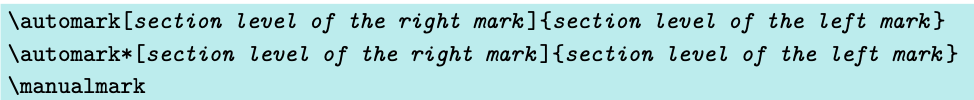
\includegraphics[width=0.9\linewidth]{imagens/imagem05.png}
\end{figure}

Tanto nas classes \LaTeX\ padrão quanto nas classes \KOMAScript\ a decisão de usar cabeçalhos automáticos ou estáticos é feita usando o estilo de página apropriado. Cabeçalhos repetem algum texto descritivo, como um título, que é apropriado para a página ou coluna, geralmente no cabeçalho, mais raramente no rodapé. Como já explicado na seção 3.12, você obtém cabeçalhos automáticos com títulos 

Nas classes de artigo \textbf{article} ou \textbf{scrartcl}, o estilo de página de títulos usa o título da seção, que é o argumento obrigatório ou opcional de \cmd{section}, para o título de documentos de um lado. Documentos de dois lados usam este título de seção como a marca esquerda e o título de subseção como a marca direita. A marca esquerda é impressa, como o nome indica, nas páginas esquerdas (verso). A marca direita é impressa nas páginas direitas (reto) — na impressão de um lado, isso significa em todas — as páginas. As classes, por padrão, também excluem a marca direita sempre que colocam o título da seção na marca esquerda.

As classes de relatório e livro começam um nível acima. Assim, elas usam o título do capítulo como a marca direita na impressão de um lado. Na impressão frente e verso, o título do capítulo é a marca esquerda e o título da seção é a marca direita.

Se você usar \texttt{myheadings}, as marcas no cabeçalho da página ainda existirão, e os números de página serão colocados da mesma forma, mas os comandos de seção não definem mais as marcas automaticamente. Você pode defini-las manualmente usando os comandos \cmd{markright} e \cmd{markboth}, que são descritos mais adiante nesta seção.

Essa distinção foi eliminada pelo \textbf{scrlayer}. Em vez de distinguir entre cabeçalhos automáticos e manuais pelo estilo de página selecionado, há dois novos comandos:
\begin{verbatim}
    \automark
    \manualmark
\end{verbatim}

O comando \cmd{manualmark} alterna para marcas manuais e desativa o preenchimento automático das marcas. Em contraste, \cmd{automark} e \cmd{automark*} definem quais níveis de seção devem ser usados para definir a marca automaticamente. O argumento opcional é o nível de seção da marca direita, o argumento obrigatório é o nível de seção da marca esquerda. Os argumentos devem sempre ser o nome de um nível de seção como parte, capítulo, seção, subseção, subsubseção, parágrafo ou subparágrafo.

Normalmente, o nível mais alto deve ser usado para a marca esquerda e o nível mais baixo para a marca direita. Isso é apenas uma convenção e não um requisito, mas faz sentido.

Observe que nem toda classe fornece cabeçalhos de execução para cada nível de seção. Por exemplo, as classes padrão nunca usam \cmd{part} no título. As classes \KOMAScript\ por outro lado, suportam todos os níveis.

A diferença entre \cmd{automark} e \cmd{automark*} é que \cmd{automark} substitui todos os comandos anteriores para definir automaticamente a marca, enquanto \cmd{automark*} altera apenas o comportamento dos níveis de seção especificados em seus argumentos.

\textbf{Exemplo}: Suponha que você queira que os títulos dos capítulos sejam usados como cabeçalho de páginas pares e o título da seção seja o cabeçalho de páginas ímpares, como de costume. Mas em páginas ímpares você também quer que os títulos dos capítulos sejam usados como cabeçalho até que a primeira seção apareça. Para fazer isso, primeiro você precisa carregar o \textbf{scrlayer-scrpage} e selecionar o estilo de página \texttt{scrheadings}, para que o documento comece com:
\begin{verbatim}
\documentclass{scrbook}
\usepackage{scrlayer-scrpage}
\pagestyle{scrheadings} 
\end{verbatim}

Em seguida, certifique-se de que os títulos dos capítulos definam as marcas da esquerda e da direita: \cmd{automark[chapter]\{chapter\}}

Então o título da seção também deve definir as marcas da direita:

\verb|\automark*[section]{}|

Aqui, a versão com estrela é usada, já que o comando \cmd{automark} anterior deve permanecer em vigor. Além disso, o argumento obrigatório para o nível de seção da marca da esquerda está vazio porque essa marca deve permanecer inalterada.

Tudo o que falta agora é um pouco de conteúdo do documento para mostrar o resultado:
\begin{verbatim}
\usepackage{lipsum}
\begin{document}
\chapter{Título do Capítulo}
\lipsum[1-20]
\section{Título da Seção}
\lipsum[21-40]
\end{document}  
\end{verbatim}

Usamos o pacote extremamente útil \textit{lipsum} para gerar algum texto fictício com comando \cmd{lipsum}.

Se você testar o exemplo, verá que a primeira página do capítulo aparece, como de costume, sem um título corrente, já que esta página usa automaticamente o estilo de página simples \texttt{plain.scrheadings} (ver sobre \cmd{chap\-ter\-pa\-ge\-sty\-le} na página 83). As páginas 2–4 têm os títulos dos capítulos no título corrente. Após o título da seção na página 4, o título corrente da página 5 muda para este título da seção. Desta página até o final, o título corrente alterna de página para página entre os títulos do capítulo e da seção.

\begin{figure}[h]
    \centering
    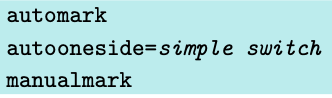
\includegraphics[width=0.5\linewidth]{imagens/imagem07.png}
\end{figure}

Em vez dos comandos descritos anteriormente, você também pode usar as opções \texttt{manualmark} e \texttt{automark} para alternar entre cabeçalhos de execução automáticos e manuais. \texttt{automark} sempre usa o padrão \cmd{automark[section]\{chapter\}} para classes com \cmd{chapter} e \cmd{automark[subsection]\{section}\} para outras classes.

Na impressão unilateral, você normalmente quer que apenas os níveis de seção mais altos forneçam o título de execução. A opção padrão \texttt{autooneside} corresponde a esse comportamento. A opção aceita os valores para interruptores simples listados na tabela 2.5, página 41. Se você desativar essa opção, os argumentos opcionais e obrigatórios de \texttt{automark} e \texttt{automark*} controlarão novamente o cabeçalho de execução na impressão unilateral.

\textbf{Exemplo}: Suponha que você tenha um relatório unilateral, mas queira títulos semelhantes aos do exemplo de livro anterior. Especificamente, os títulos dos capítulos devem ser usados como título até que a primeira seção apareça. Daí em diante, o título da seção deve ser usado. Então, modificamos um pouco o exemplo anterior:
\begin{verbatim}
\documentclass{scrreprt}
\usepackage[autooneside=false]{scrlayer-scrpage}
\pagestyle{scrheadings}
\automark[section]{chapter}
\usepackage{lipsum}
\begin{document}
\chapter{Título do capítulo}
\lipsum[1-20]
\section{Título da seção}
\lipsum[21-40]
\end{document}    
\end{verbatim}

Como você pode ver, um comando \texttt{automark*} não é necessário neste caso. Você deve tentar o exemplo com \texttt{autooneside} definido como \textit{true} ou remover a opção para comparação. Você notará uma diferença no cabeçalho de execução da página 4 em diante.
Note que apenas carregar o pacote não tem efeito algum sobre se cabeçalhos de execução automáticos ou manuais são usados, ou que tipo de cabeçalhos de seccionamento preenchem as marcas. Somente usando explicitamente a opção \texttt{automark} ou \texttt{manualmark}, ou o comando \cmd{automark} ou \cmd{manualmark}, as condições aqui serão inicializadas.

\begin{figure}[h]
     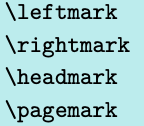
\includegraphics[width=0.2\linewidth]{imagens/imagem08.png}
\end{figure}

Se você quiser se afastar dos estilos de página predefinidos, normalmente precisa decidir onde colocar o conteúdo das marcas. Com \cmd{left\-mark} você pode definir o que aparecerá na marca esquerda quando a página for impressa.

Da mesma forma, você pode usar \cmd{right\-mark} para definir o conteúdo da marca direita.

Você pode facilitar a vida com \cmd{headmark}. Esta extensão do \textbf{scrlayer} é uma abreviação que resolve para \cmd{left\-mark} ou \cmd{right\-mark} dependendo se a página atual é par ou ímpar.

O comando \cmd{pagemark} não tem nada a ver com o mecanismo de marca do TeX. Ele é usado para exibir um número de página formatado. A fonte do elemento \texttt{pagenumber} será usada para a saída. Isso pode ser alterado usando os comandos \cmd{set\-ko\-ma\-font} ou \cmd{add\-to\-ko\-ma\-font} (veja também a seção 3.6, página 58).

\textbf{Exemplo}: Suponha que você queira que o cabeçalho seja alinhado à margem esquerda e o número da página à margem direita na impressão unilateral. O seguinte exemplo mínimo de trabalho faz exatamente isso:
\begin{verbatim}
\documentclass{scrreprt}
\usepackage{blindtext}
\usepackage[automark]{scrlayer-scrpage}
\pagestyle{scrheadings}
\ihead{\headmark}
\ohead*{\pagemark}
\chead{}
\cfoot[]{}
\begin{document}
\blinddocument
\end{document}  
\end{verbatim}

O pacote \texttt{blindtext} e seu comando \cmd{blind\-do\-cu\-ment} foram usados aqui para gerar rapidamente o conteúdo do documento de amostra para o exemplo.

Os comandos \cmd{ihead} e \cmd{ohead*} configuram as marcas desejadas. A variante \cmd{ohead*} com estrela também configura o número da página com o estilo de página \texttt{plain.scrheadings} usado na primeira página de um capítulo.

Como esses estilos de página têm marcas predefinidas no centro do cabeçalho e rodapé, esses elementos são limpos usando \cmd{chead} e \cmd{cfoot} com argumentos vazios. Como alternativa, você pode usar \cmd{clear\-pair\-of\-pa\-ge\-sty\-les} antes de \cmd{ihead}. Você encontrará esse comando descrito na seção 18.2.

Observe que o argumento opcional vazio de \cmd{cfoot} no exemplo acima não é o mesmo que omitir o argumento opcional. Você deve tentar você mesmo e dar uma olhada na diferença no rodapé da primeira página.

Usuários avançados podem encontrar mais comandos de configuração de marca a partir da página 448.

\begin{figure}[h]
    \centering
    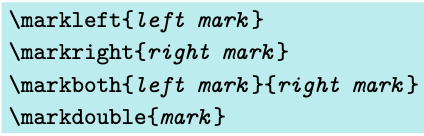
\includegraphics[width=0.5\linewidth]{imagens/imagem09.png}
\end{figure}

Independentemente de você estar trabalhando com cabeçalhos de execução manuais ou automáticos, você pode sempre alterar o conteúdo da marca esquerda ou da marca direita usando esses comandos. Observe que a marca à esquerda resultante de \cmd{leftmark} será a última marca colocada na página correspondente, enquanto a marca à direita resultante de \cmd{rightmark} é a primeira marca colocada na página correspondente. Para mais detalhes, consulte \cmd{ri\-ght\-first\-mark} na seção 17.6, página 443.

Se você estiver usando cabeçalhos de execução manuais, as marcas permanecerão válidas até que sejam explicitamente substituídas pela reutilização dos comandos correspondentes. No entanto, se você estiver usando cabeçalhos de execução automáticos, as marcas podem se tornar inválidas com o próximo título de seção, dependendo da configuração automática.

Você também pode usar esses comandos em conjunto com as versões com estrela dos comandos de seção.

\textbf{Exemplo}: Suponha que você escreva um prefácio de várias páginas colocadas logo antes do índice mas não aparecendo nele. No entanto, como você usa linhas divisórias no seu cabeçalho, você quer um cabeçalho para este prefácio:
\begin{verbatim}
\documentclass[headsepline]{book}
\usepackage{scrlayer-scrpage}
\pagestyle{scrheadings}
\usepackage{blindtext}
\begin{document}
\chapter*{Preface}
\markboth{Preface}{Preface}
\blindtext[20]
\tableofcontents
\blinddocument
\end{document}    
\end{verbatim}

À primeira vista, isso parece produzir o resultado desejado. Dando uma segunda olhada, no entanto, você pode ver que o título “Preface” não aparece em letras maiúsculas, ao contrário dos outros cabeçalhos. Mas isso é fácil de mudar:
\begin{verbatim}
\documentclass[headsepline]{book}
\usepackage{scrlayer-scrpage}
\pagestyle{scrheadings}
\usepackage{blindtext}
\begin{document}
\chapter*{Preface}
\markboth{\MakeMarkcase{Preface}}{\MakeMarkcase{Preface}}
\blindtext[20]
\tableofcontents
\blinddocument
\end{document}   
\end{verbatim}

Usar o comando \cmd{MakeMarkcase} resulta na obtenção da mesma caixa de letras que para cabeçalhos de execução automáticos.

Agora, vamos mover o \cmd{tableofcontents} para a frente do prefácio e remover o comando \cmd{markboth}. Você descobrirá que o prefácio agora tem o cabeçalho de execução “CONTENTS”. Isso se deve a uma peculiaridade do \cmd{chapter*} (veja também a seção 3.16 na página 105).

Se você não quiser um cabeçalho de execução aqui, você pode facilmente fazer isso passando dois argumentos vazios para \cmd{markboth}:
\begin{verbatim}
\documentclass[headsepline]{book}
\usepackage{scrlayer-scrpage}
\pagestyle{scrheadings}
\usepackage{blindtext}
\begin{document}
\tableofcontents
\chapter*{Preface}
\markboth{}{}
\blindtext[20]
\blinddocument
\end{document}    
\end{verbatim}

O comando \cmd{markdouble} altera a marca esquerda e a marca direita para o mesmo conteúdo. Então \cmd{mark\-dou\-ble\{mark\}} é uma forma mais curta de \cmd{mark\-both\{mark\}\-\{mark\}} com dois argumentos idênticos.

